\documentclass[../ManualeSviluppatore.tex]{subfiles}

\begin{document}
\section{Database}
	\subsection{Schema ER}
		\begin{figure} [h]
				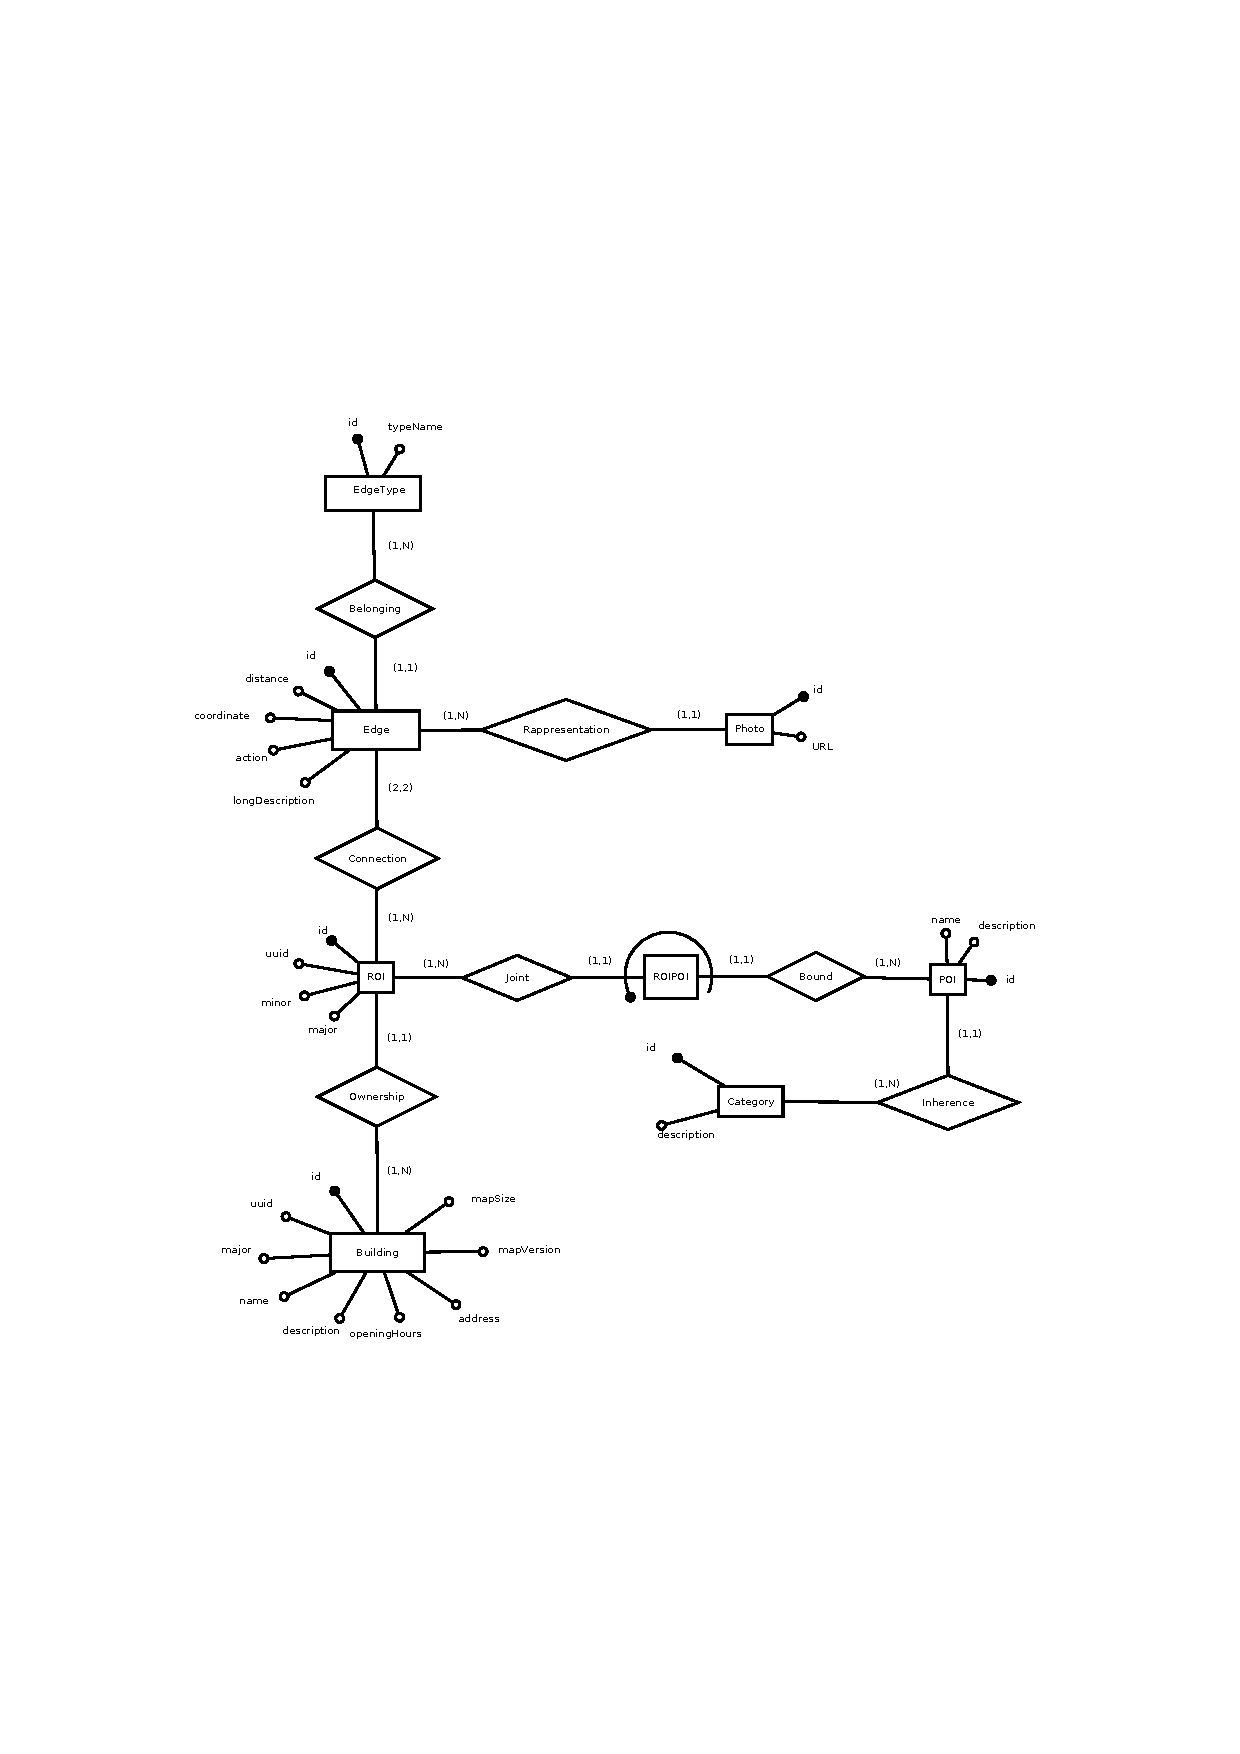
\includegraphics[width=\textwidth]{img/Database}		
				\caption{Schema ER - base di dati}
				\label{Database}
		\end{figure}
	\subsection{Descrizione relazioni}
		\subsubsection{Building}
		Relazione che contiene le informazioni degli edifici. Attributi:
		\begin{itemize}
			\item \textbf{id}: chiave primaria, intero;
			\item \textbf{uuid}: stringa, rappresenta l'identificativo UUID uguale per tutti i beacon utilizzati dall'applicazione;
			\item \textbf{major}: intero, rappresenta l'identificativo Major uguali per tutti i beacon di uno stesso edificio, chiave esterna verso la relazione Building;
			\item \textbf{name}: stringa, rappresenta il nome dell'edificio;
			\item \textbf{description}: stringa, rappresenta la descrizione dell'edificio e delle sue funzionalità;
			\item \textbf{openingHours}: stringa, rappresenta gli orari di apertura dell'edificio;
			\item \textbf{address}: stringa, rappresenta l'indirizzo dell'edificio;
			\item \textbf{mapVersion}: stringa, rappresenta la versione della mappa;
			\item \textbf{mapSize}: stringa, rappresenta la dimensione della mappa.
		\end{itemize}
		\subsubsection{ROI}
		Relazione che contiene le informazioni delle Region of interest. Attributi:
			\begin{itemize}
			\item \textbf{id}: chiave primaria, intero;
			\item \textbf{uuid}: stringa, rappresenta l'identificativo UUID uguale per tutti i beacon utilizzati dall'applicazione;
			\item \textbf{major}: intero, rappresenta l'identificativo Major uguali per tutti i beacon di uno stesso edificio;
			\item \textbf{minor}: intero, rappresenta l'identificativo Minor che identifica univocamente un beacon in un edificio.
			\end{itemize}
		\subsubsection{ROIPOI}
		Relazione che contiene le associazioni tra Region of interest e Point of interest. Attributi:
			\begin{itemize}
			\item \textbf{idRoi}: intero, chiave esterna verso la relazione ROI;
			\item \textbf{idPoi}: intero, chiave esterna verso la relazione POI;
			\item chiave primaria (idRoi, idPoi).
			\end{itemize}
		\subsubsection{POI}
		Relazione che contiene le informazioni dei Point of interest. Attributi:
			\begin{itemize}
			\item \textbf{id}: chiave primaria, intero;
			\item \textbf{name}: string, rappresenta il nome associato al Point of interest;
			\item \textbf{description}: stringa, rappresenta la descrizione del Point of interest.
			\end{itemize}
		\subsubsection{Category}
		Relazione che contiene le informazioni delle categorie di Point of interest. Attributi:
			\begin{itemize}
			\item \textbf{id}: chiave primaria, intero;
			\item \textbf{description}: stringa, rappresenta la descrizione della categoria di Point of Interest.
			\end{itemize}
		\subsubsection{Edge}
		Relazione che contiene le informazioni delle connessioni tra le Region of interest, che rappresentano gli archi del grafo che rappresenta un edificio. Attributi:
			\begin{itemize}
			\item \textbf{id}: chiave primaria, intero;
			\item \textbf{distance}: intero, rappresenta la lunghezza dell'arco;
			\item \textbf{coordinate}: string, rappresenta l'ampiezza dell'arco che ha per lati l'arco e il collegamento tra la Region Of Interest di partenza e il nord polare; 
			\item \textbf{action}: string, rappresenta le azioni che bisogna compiere per superare l'arco;
			\item \textbf{longDescription}: string, rappresenta una descrizione dettagliata delle azioni che bisogna compiere per superare l'arco;
			\item \textbf{startROI}: intero, chiave esterna verso la relazione ROI, rappresenta la Region of interest di partenza dell'arco;
			\item \textbf{endROI}: intero, chiave esterna verso la relazione ROI, rappresenta la Region of interest di arrivo dell'arco.
			\end{itemize}
		\subsubsection{EdgeType}
		Relazione che contiene le informazioni sui tipi degli archi. Attributi:
			\begin{itemize}
			\item \textbf{id}: chiave primaria, intero;
			\item \textbf{typeName}: stringa, rappresenta la descrizione del tipo di arco.
			\end{itemize}
		\subsubsection{Photo}
		Relazione che contiene i link alle immagini associati ad un arco. Attributi:
			\begin{itemize}
			\item \textbf{id}: chiave primaria, intero;
			\item \textbf{URL}: stringa, rappresenta l'URL a cui recuperare l'immagine;
			\item \textbf{edgeId}: intero, chiave esterna verso la relazione Edge, rappresenta l'Edge a cui è associata l'immagine.
			\end{itemize}
	\subsection{Descrizione associazioni}
		\subsubsection{Ownership}
			Associazione che unisce ogni ROI all'edificio di appartenenza.\\
			\textbf{Molteplicità}:(1,N) Ad ogni Building possono essere associati uno o più ROI, ogni ROI può essere associato un solo edificio.

		\subsubsection{Connection}
			Associazione che unisce ogni Edge ai ROI di partenza e arrivo. \\
			\textbf{Molteplicità}:(2,N) Ad ogni Edge associa il ROI di inizio e fine, ogni ROI può essere associato ad uno o più Edge.

		\subsubsection{Joint}
			Associazione che unisce ogni ROI ai ROIPOI di appartenenza. \\
			\textbf{Molteplicità}:(1,N) Ogni ROI può essere associato ad uno o più ROIPOI, ogni ROIPOI può essere associato ad un unico ROI.

		\subsubsection{Bound}
			Associazione che unisce ogni POI ai ROIPOI di appartenenza. \\
			\textbf{Molteplicità}:(1,N) Ogni POI può essere associato ad uno o più ROIPOI, ogni ROIPOI può essere associato ad un unico POI.

		\subsubsection{Inherence}
			Associazione che unisce ogni POI alla categoria a cui appartiene.\\
			\textbf{Molteplicità}:(1,N) Ogni POI può essere associato ad una unica Category, ogni Category può essere associata a più POI.

		\subsubsection{Rappresentation}
			Associazione che unisce ogni Photo all'Edge che rappresenta. \\
			\textbf{Molteplicità}:(1,N) Ogni Photo può essere associata ad un unico Edge, ogni Edge può avere più Photo.

		\subsubsection{Belonging}
			Associazione che unisce ogni Edge al tipo a cui appartiene.\\
			\textbf{Molteplicità}:(1,N) Ogni Edge può essere associato ad un unico EdgeType, ogni EdgeType può essere associato ad uno o più Edge.

\end{document}